
\chapter{Menu Surfaces}
\minitoc 


In most cases, these function only apply on selected surfaces, so, as a prerequisite, you almost always need to select surfaces in order to use what is described below.



\section{Structure modification}
\subsection{Smooth each selected surface}
\noindent
\begin{minipage}{0.5\textwidth}
This option uses vtkSmoothPolyDataFilter.You may smooth an input
selected surface using this option (see Fig. \ref{smooth}). A number of iteration and a
relaxation factor are required.\\
See vtkSmoothPolyDataFilter documentation for further information regarding this option.
\end{minipage}    
\begin{minipage}{0.5\textwidth}\centering
  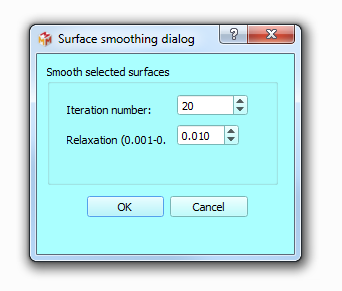
\includegraphics[scale=0.5]{images/09/structure/surface_smoothing_dialog.png}
 \captionof{figure}{Surface smoothing dialog}
 \end{minipage} 
\noindent

\begin{figure}
  \centering
  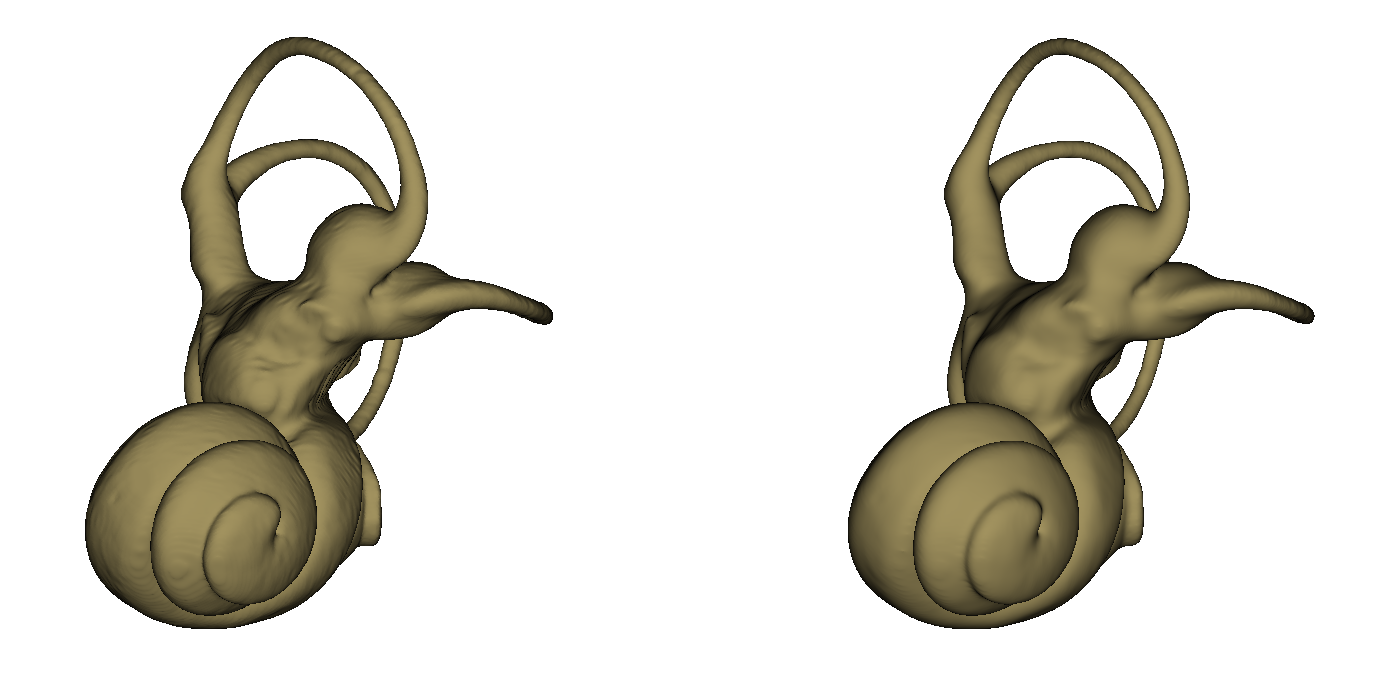
\includegraphics[scale=0.35]{images/09/structure/surface_smoothing_example.png} 
	\caption{Smoothing surfaces. Left: example of original input surface (left inner ear of \textit{Galago moholi}). Right: resulting output surface after 100 iterations using a relaxation factor of 0.1.}
\label{smooth}
 
\end{figure}





\subsection{Decimate each selected surface}
\noindent
\begin{minipage}{0.5\textwidth}


This option uses vtkDecimatePro and vtkQuadricDecimation filters. Requirements : to use mesh decimation, a selected
surface is required (see for instance Fig. \ref{decimate}). See vtkDecimatePro and vtkQuadricDecimation documentations for further information regarding
mesh decimation.

\end{minipage}    
\begin{minipage}{0.5\textwidth}\centering
  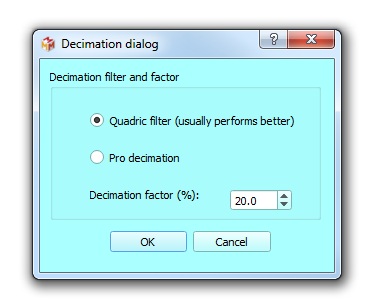
\includegraphics[scale=0.5]{images/09/structure/decimation_dialog.png}
 \captionof{figure}{Decimate window}
 \end{minipage} 
\noindent

\begin{figure}
  \centering
  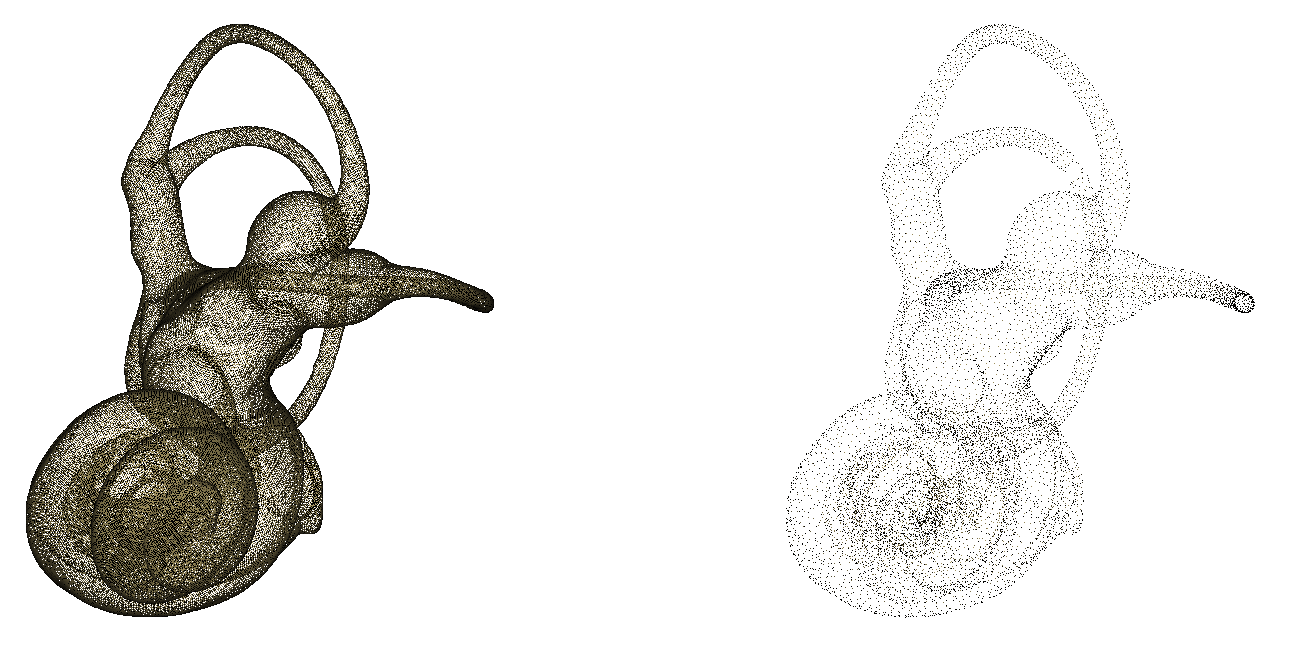
\includegraphics[scale=0.35]{images/09/structure/decimation_example.png} 
	\caption{Surface decimation. Left: point cloud rendering of input surface (left inner ear of \textit{Galago moholi}). Right: point cloud rendering of resulting output (vtkQuadricDecimation filter,
decimation factor: 95\%). 
}
\label{decimate}
 
\end{figure}

\subsection{Densify each selected surface}

\noindent
\begin{minipage}{0.5\textwidth}

This option uses vtkDensifyPolyData filter.
Requirements : to use mesh densification, a selected
surface is required (see for instance Fig. \ref{densify}).
Note that mesh decimation can become extremely slow
when using number of subdivisions larger than 1.
See vtkDensifyPolyData documentation for further information regarding mesh densification.

\end{minipage}    
\begin{minipage}{0.5\textwidth}\centering
  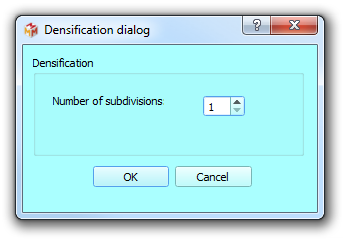
\includegraphics[scale=0.5]{images/09/structure/densification_dialog.png}
 \captionof{figure}{Densify dialog}
 \end{minipage} 
\noindent

\begin{figure}
  \centering
  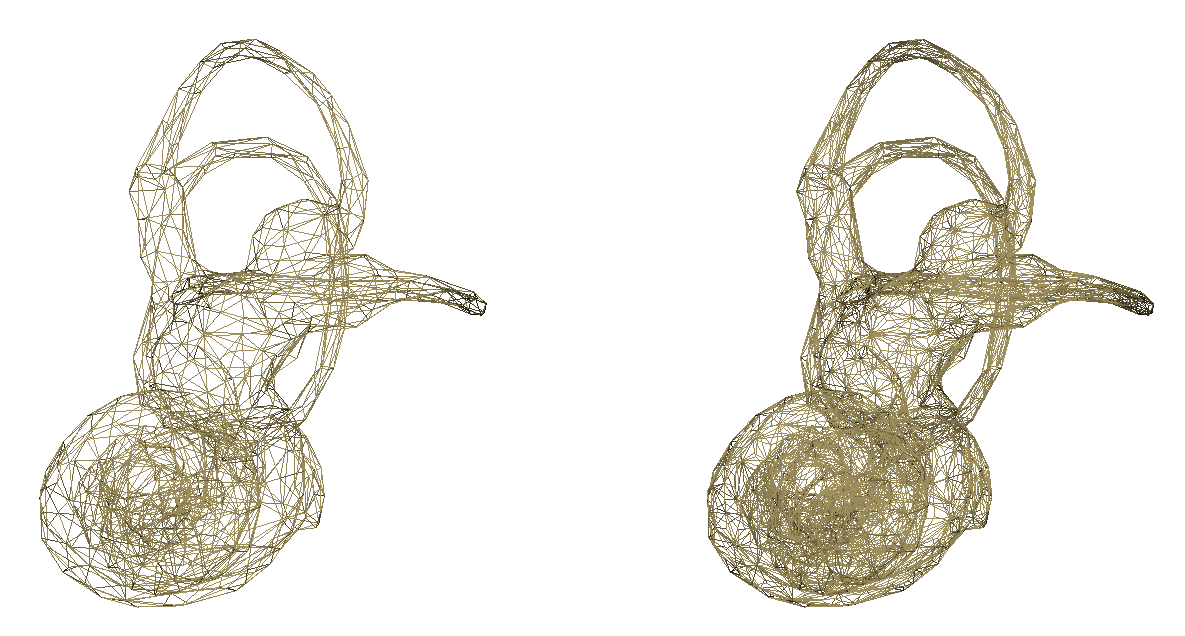
\includegraphics[scale=0.35]{images/09/structure/densification_example.png} 
	\caption{Surface densification. Left: wireframe rendering of input surface (left inner ear of \textit{Galago moholi}). Right: wireframe rendering of resulting output (number of subdivisions: 1).
}
\label{densify}
 
\end{figure}




\subsection{Fill holes of each selected surface}

\noindent
\begin{minipage}{0.5\textwidth}

This option uses vtkFillHolesFilter.
Requirements : to use mesh hole filling, a selected surface is
required (see for instance Fig. \ref{fill_holes}). See vtkFillHolesFilter documentation for further
information regarding hole filling.


\end{minipage}    
\begin{minipage}{0.5\textwidth}\centering
  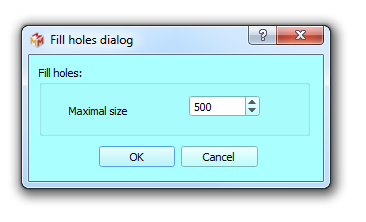
\includegraphics[scale=0.5]{images/09/structure/fill_holes_dialog.png}
 \captionof{figure}{Fill holes window}
 \end{minipage} 
\noindent

\begin{figure}
  \centering
  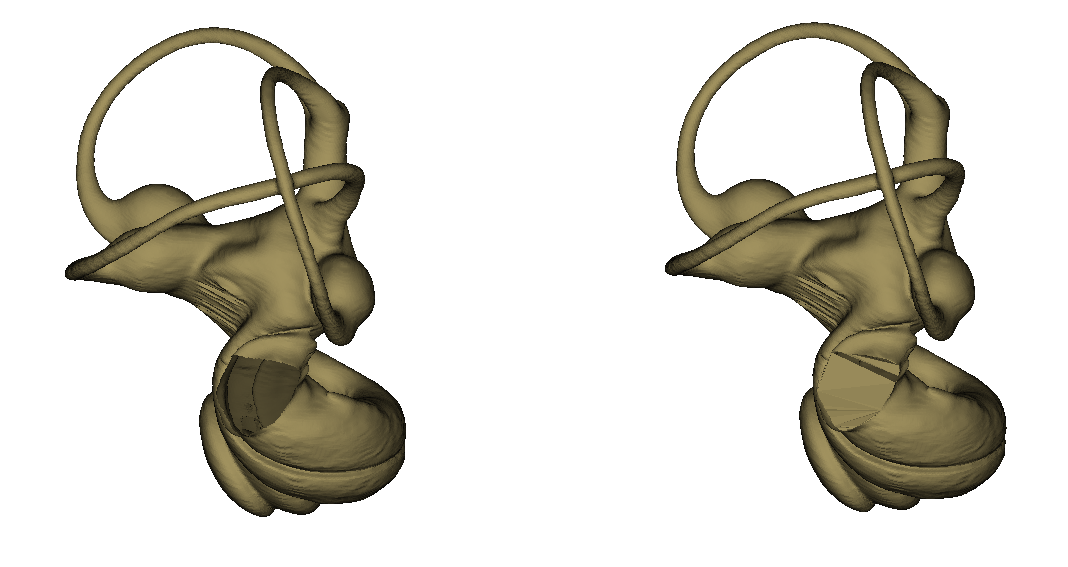
\includegraphics[scale=0.35]{images/09/structure/fill_holes_example.png} 
	\caption{Filling holes. Left: input surface: left inner ear of \textit{Galago moholi} having a hole in the round window. Right: resulting surface output.}
\label{fill_holes}
 
\end{figure}






\subsection{TPS deformation of each selected surface}
\noindent
\begin{minipage}{0.5\textwidth}
This option uses vtkThinPlateSplineTransform filter.
Requirements : to use TPS deformation, a selected surface,
a series of ``n" normal landmarks and a series of ``n"
target landmarks (n>3) are needed. ``Normal" landmarks
are usually placed on the original selected input surface,
whereas ``target" landmarks are placed at a location in 3D
space which will drive the TPS deformation (see Fig. \ref{tps}). See vtkThinPlateSplineTransform documentation for further information regarding TPS deformation.

\end{minipage}    
\begin{minipage}{0.5\textwidth}\centering
  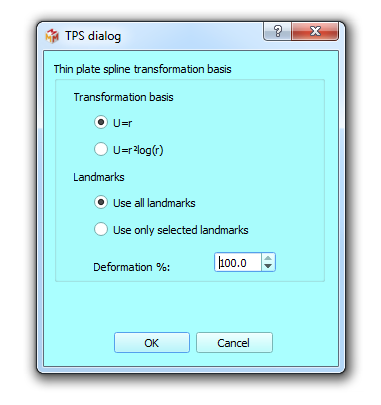
\includegraphics[scale=0.5]{images/09/structure/tps_dialog.png}
 \captionof{figure}{TPS dialog}
 \end{minipage} 
\noindent

\begin{figure}
  \centering
  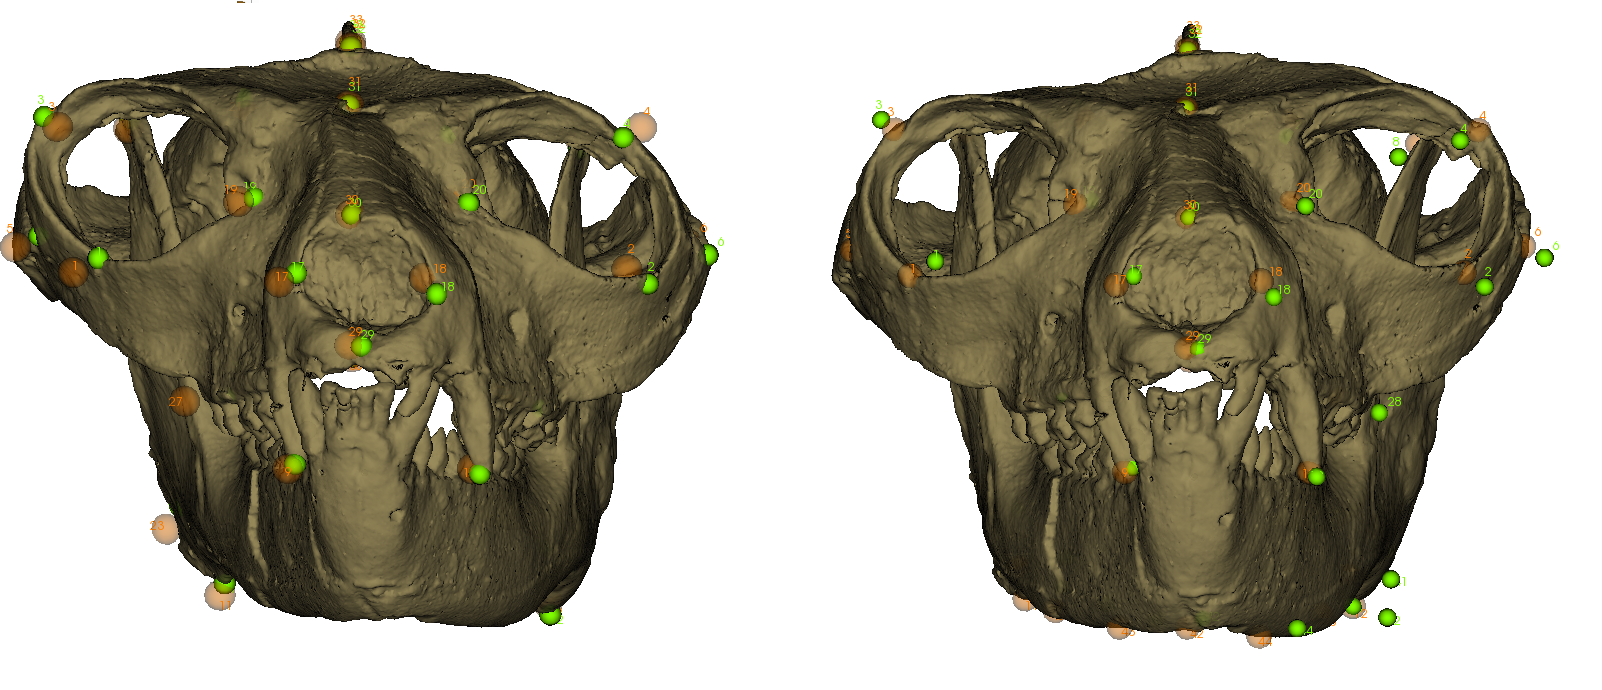
\includegraphics[scale=0.31]{images/09/structure/tps_example.png} 
	\caption{Left: original distorted input surface of the cranium and mandible of \textit{Notharctus tenebrosus} (3D surface obtained from a cast of speciman AMNH 127167 from the American Museum of Natural History, New York City, New York, USA). 46 ``normal"
landmarks were placed on the surface and 46
``target" landmarks were placed in order to
restore bilateral symmetry. Right: resulting output (deformation : 100\%). Note
that the 46 ``target" landmarks are located on the output surface.
}
\label{tps}
 
\end{figure}




\subsection{Connectivity: separate each selected surface into independent regions}
\noindent
\begin{minipage}{0.5\textwidth}
This option uses vtkPolyDataConnectivityFilter. This filter produces a new surface for each non-connected region of the selected input surface. 3D meshes of biological objects sometimes contain a multitude of small and biologically irrelevant independent regions. This ``noise" may have multiple origins: low quality of original 3D data, state of preservation of the specimen, threshold used to be able to visualize all relevant structures, etc... In order to extract relevant independent regions, only regions reaching a minimal size (minimal number of triangles) are transformed into new surfaces (see Fig. \ref{decompose34}). This process may take some time to be completed. All produced surfaces corresponding to independent regions can be manipulated independently.\end{minipage}    
\begin{minipage}{0.5\textwidth}\centering
  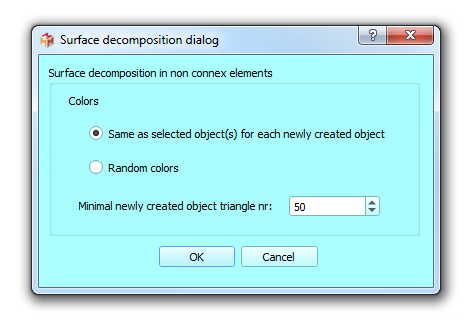
\includegraphics[scale=0.5]{images/09/structure/surface_decomposition_dialog.png}
 \captionof{figure}{Connectivity decomposition dialog}
 \end{minipage} 
\noindent


\begin{figure}
  \centering
  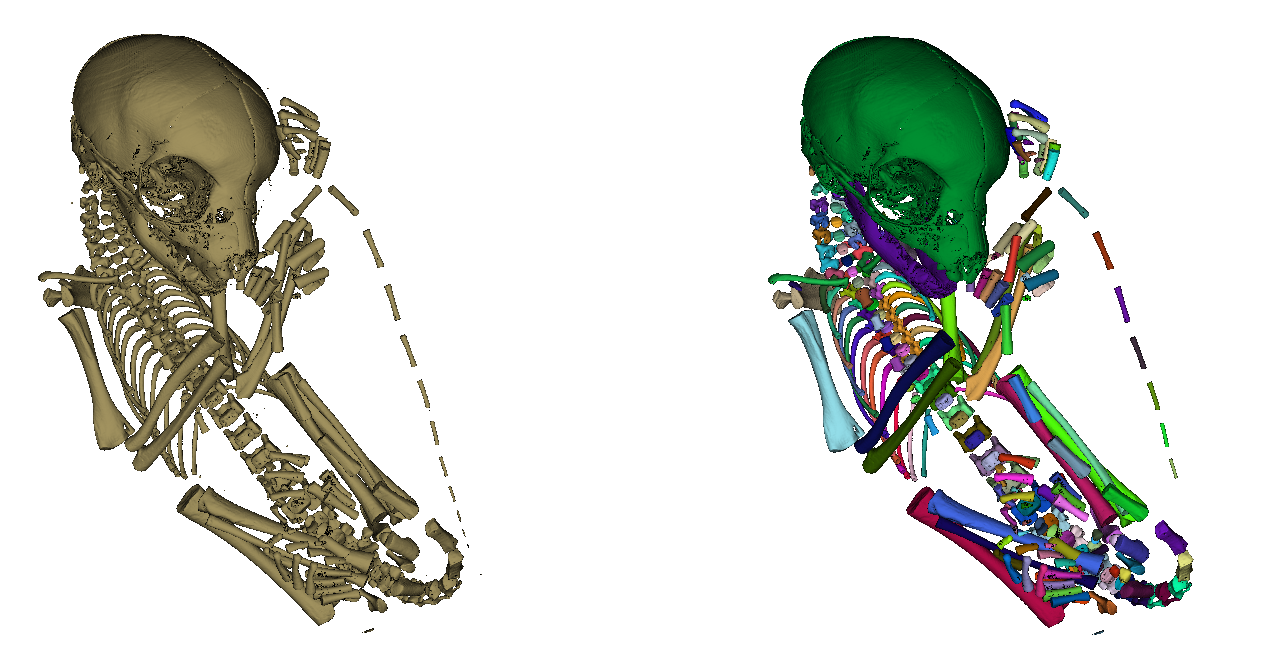
\includegraphics[scale=0.35]{images/09/structure/surface_decomposition_example.png} 
	\caption{Left: original surface of the skeleton of a newborn \textit{Lemur catta} containing a large number of independent regions of size greater than 500 triangles. Right : Output result (independent surface objects) Filtered surfaces. All surfaces produced using this filter have more than 500 triangles and were given a random color. Note that several bones of the most distal part of the tail are absent, because they contain less than 500 triangles. }
\label{decompose34}
 
\end{figure}






\subsection{Connectivity: keep largest region for each selected surface}
This option uses vtkPolyDataConnectivityFilter.This filter produces a new surface for the largest independent region of the selected input surface (see Fig. \ref{largest_region}).

\begin{figure}
  \centering
  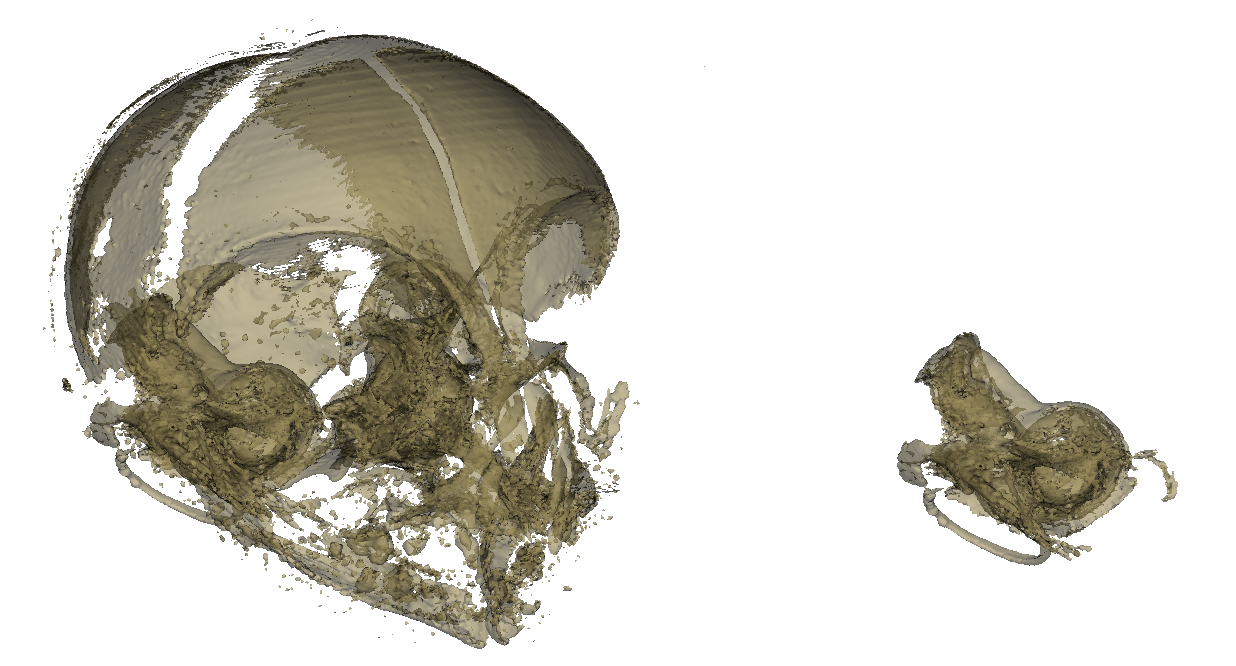
\includegraphics[scale=0.31]{images/09/structure/keep_largest.png} 
	\caption{Left: original 3D surface representing the skull of a newborn \textit{Tarsius bancanus}. Right: the resulting largest region in terms of triangle number.}
\label{largest_region}
 
\end{figure}


\subsection{Invert each selected surface}

A given surface can be inverted in order to show inner structures (see Fig. \ref{inversion}).\\


\begin{figure}
  \centering
  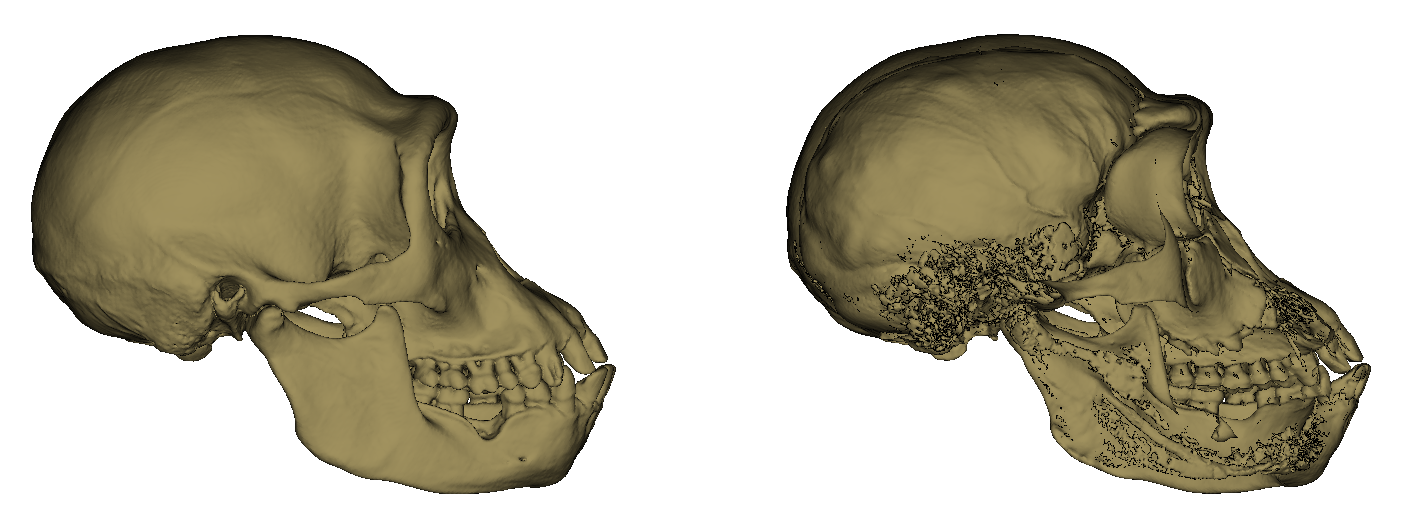
\includegraphics[scale=0.32]{images/09/structure/inversion_example.png} 
	\caption{Example of surface inversion. Left: original surface of the skull of the type specimen of \textit{Pan paniscus}.
Right: backface culling rendering of the same surface after being inverted, revealing inner structures such as the endocranial cavity. }
\label{inversion}
 
\end{figure}

\subsection{Mirror each selected surface along Y plane}

This option uses vtkReflectionFilter, which produces a mirror image of the original selected input mesh (see Fig. \ref{mirror}).\\

\begin{figure}
  \centering
  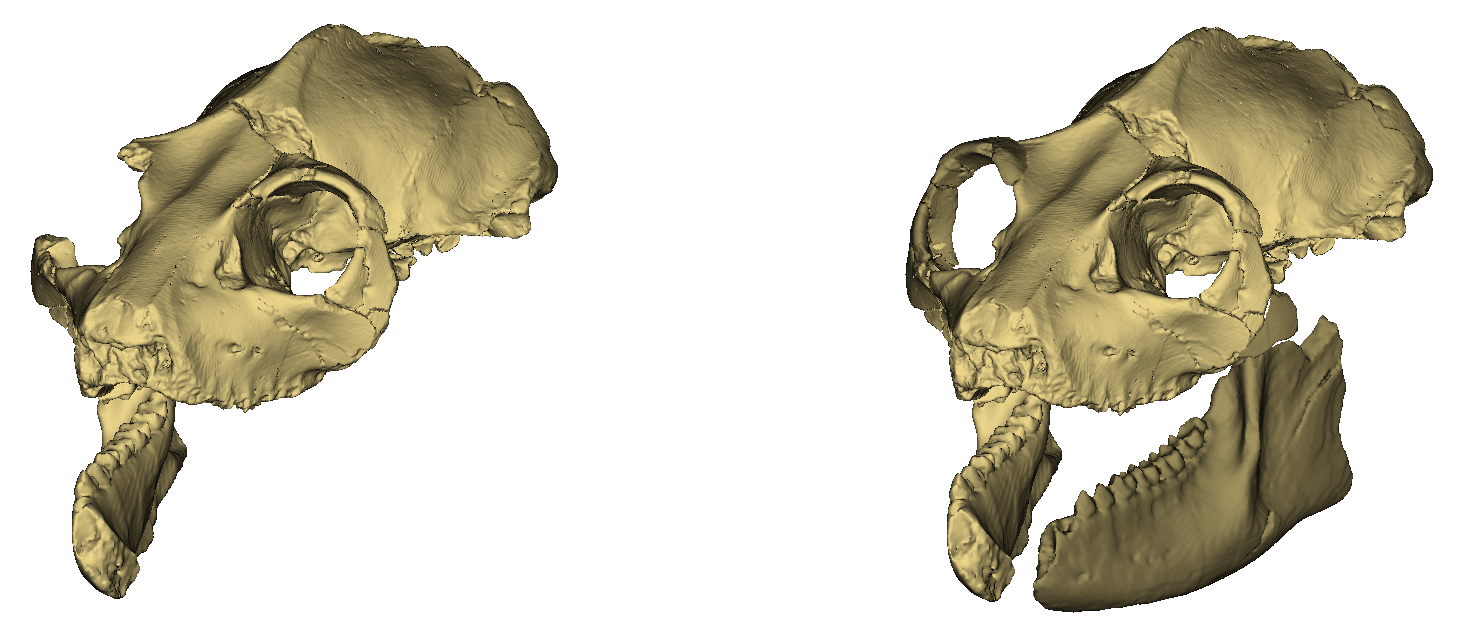
\includegraphics[scale=0.32]{images/09/structure/image_mirror.png} 
	\caption{Example of fossil restoration (\textit{Palaeolemur betillei} BOR613 specimen from the Musée d'Histoire Naturelle de Bordeaux, France) implicating the production of mirror images of missing parts.}
 \label{mirror}
\end{figure}






\subsection{Create a convex hull for each selected surface}
\subsection{Group selected surfaces}

\section{Surface alignment}
\section{Rendering modification}
\subsection{Set alpha value}
\noindent
\begin{minipage}{0.5\textwidth}

A selected surface is needed.\\
Please chose a value between 0 and 100. 100 stands for ``opaque
rendering". 0 stands for ``invisible surface".\\


\end{minipage}    
\begin{minipage}{0.5\textwidth}\centering
  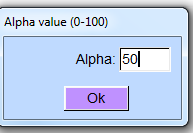
\includegraphics[scale=0.5]{images/Edit_selected_objects/10_transparency.png}
 \captionof{figure}{Alpha value setting window}
 \end{minipage} 
\noindent




As stated earlier, vertex display order has consequences on 3D rendering when working with
transparency. 3D objects are displayed one after the other following an object list. The way object are ordered inside this list thus affects transparency rendering, especially when some objects such as inner structures are positioned inside others. Object display order of selected objects can be changed using the two following controls. Pressing ``
\includegraphics[scale=0.7]{images/pixmap/s_dessous_17.png}" will place all selected objects one step earlier in the object display list. Pressing ``
\includegraphics[scale=0.7]{images/pixmap/s_dessus_17.png}" will place all selected objects one step further in the object display
list (see for instance Fig. \ref{transparency}). \\

See also ``Sort vertices from back to front (beware: slow rendering)"  (section \ref{sort_back_front}) and ``Sort vertices from front to back (beware: slow rendering)" (section \ref{sort_front_back}) for further information.\\

\begin{figure}
  \centering
  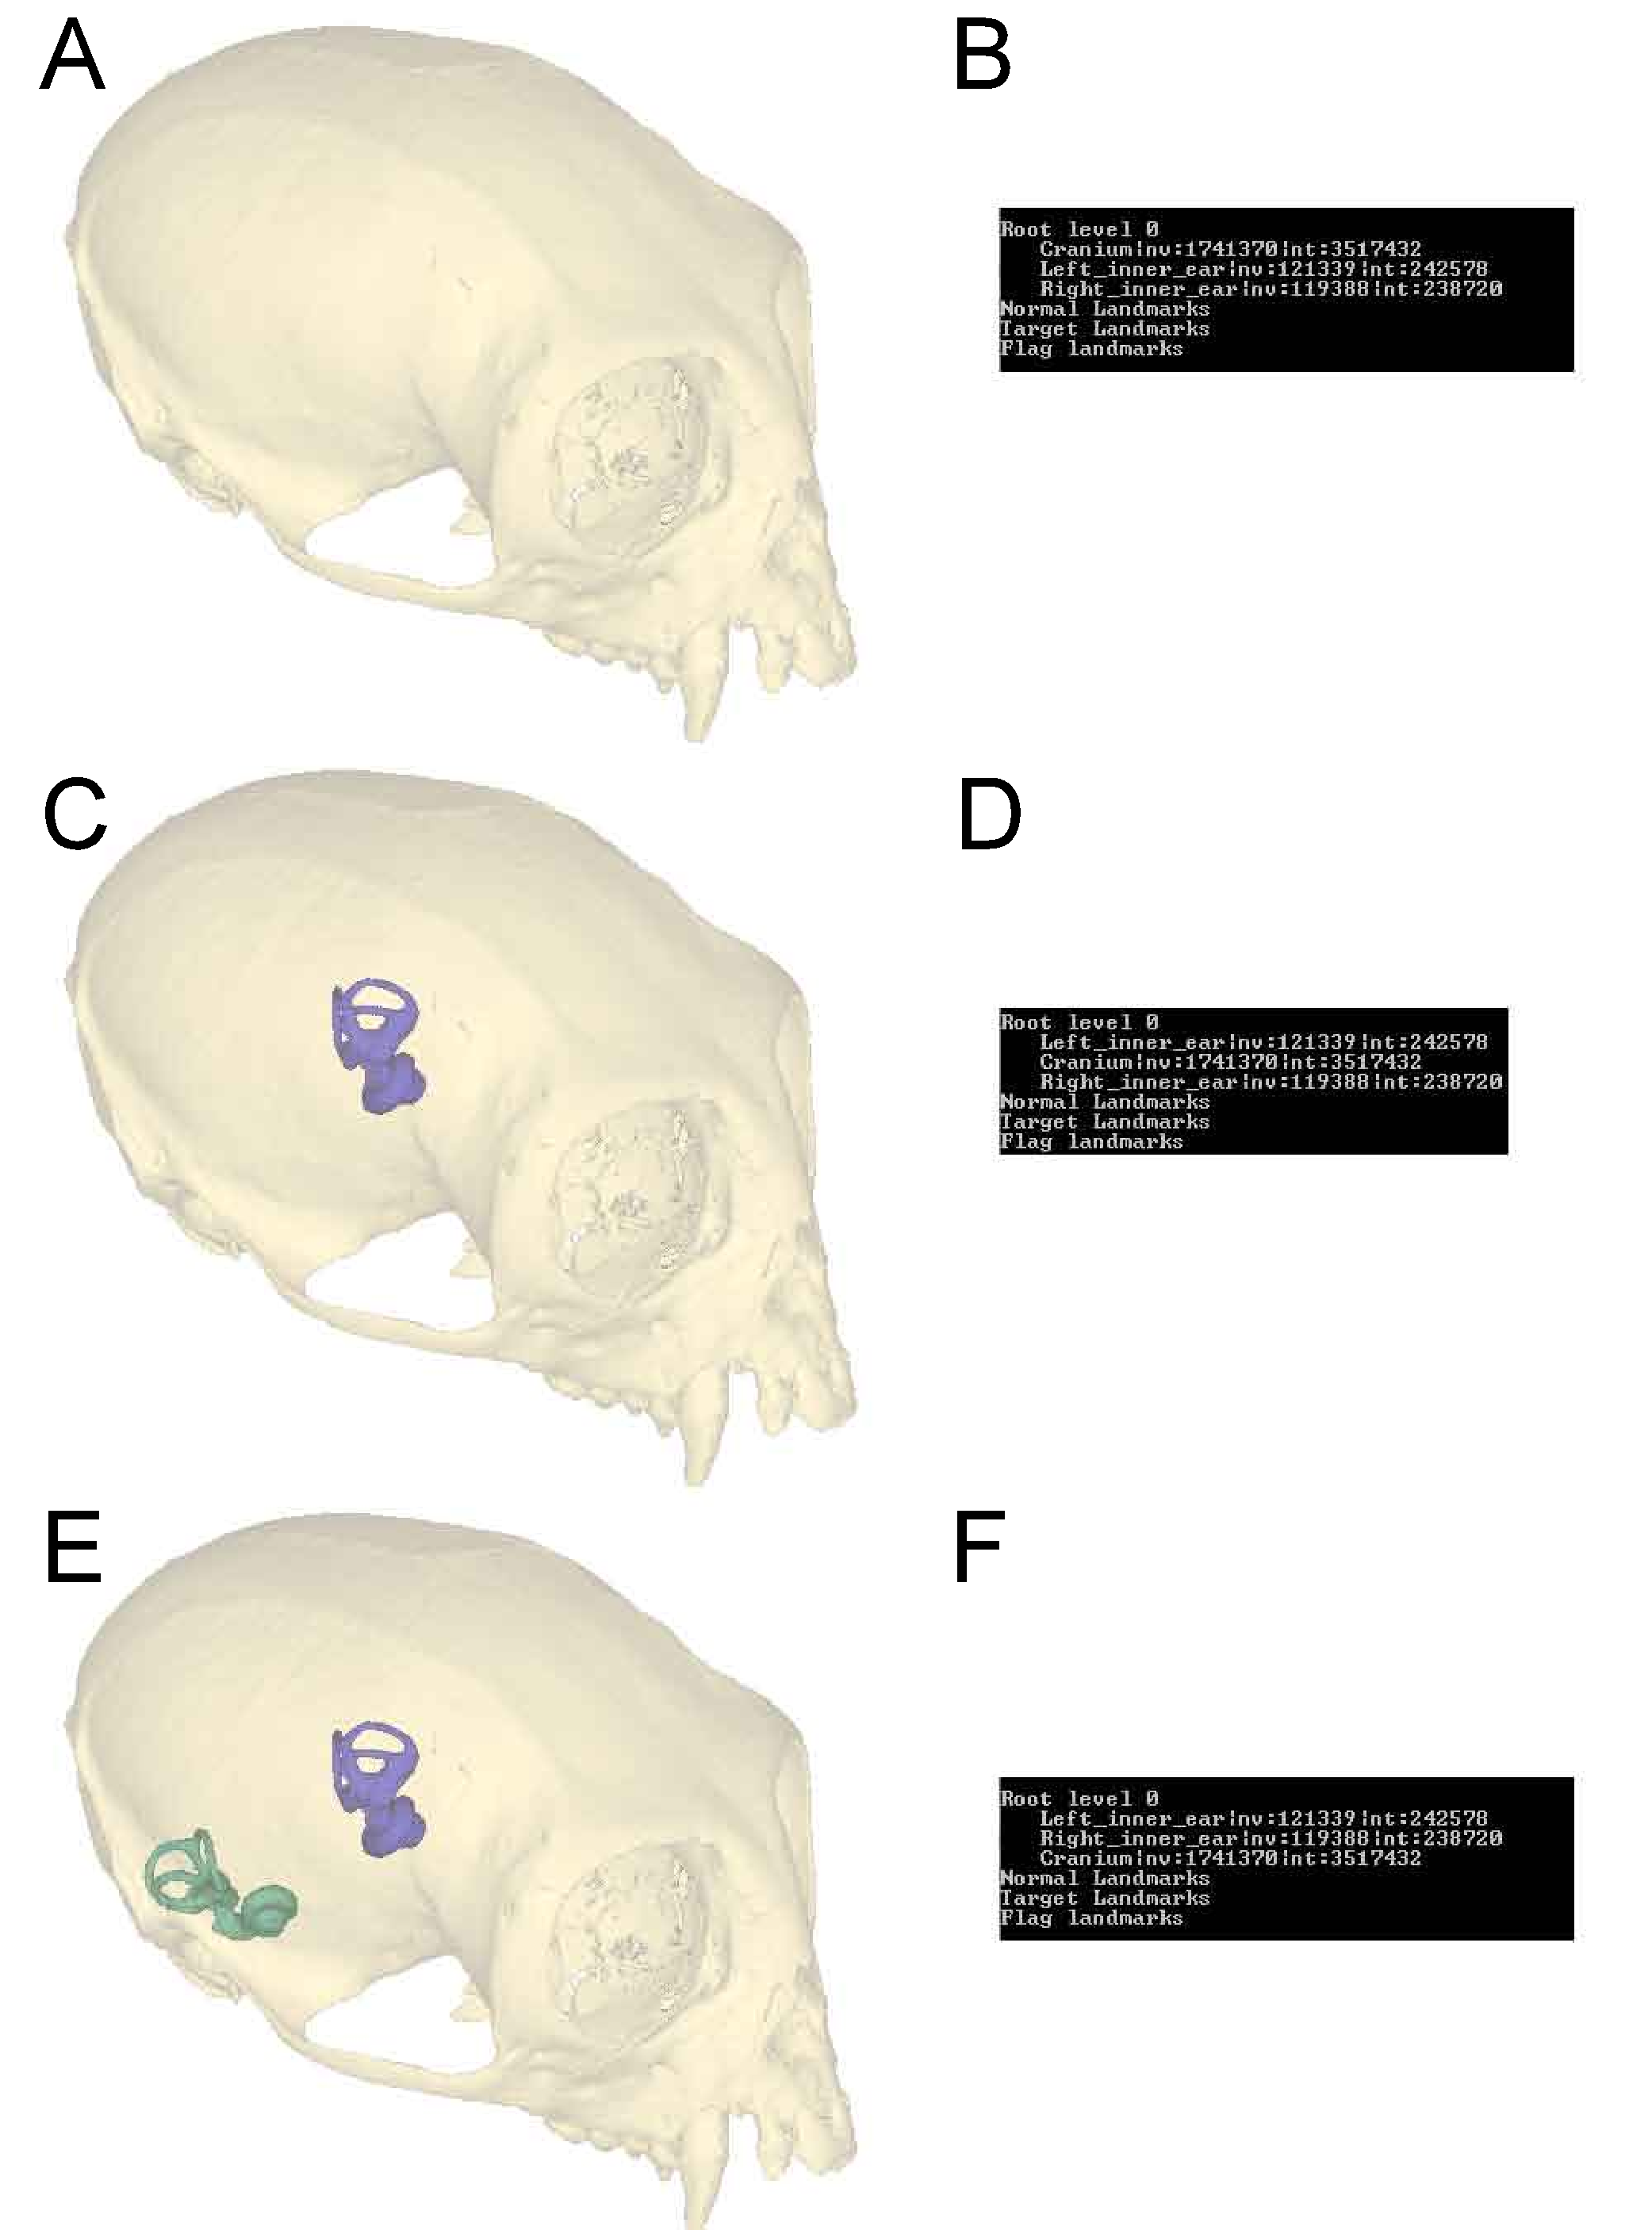
\includegraphics[scale=0.4]{images/Transparency/Transparency.pdf} 
	\caption{Transparency rendering. A. 3 objects (cranium, left\_inner\_ear and right\_
inner\_ear) are opened in this order, and the object ``cranium" is rendered with an alpha value of 40.
The inner ears remain invisible, because ``cranium" is displayed before the two inner ears are. B: corresponding display object order (Show $\rightarrow$Display
object order). C: the object ``Cranium" was selected and put downward in the object display list. Now the left inner ear is visible, as it is displayed before the cranium is. D: corresponding display object order. E: the object ``Cranium" was selected again, and put downward in the object display list. Now the two inner ears are
visible, because they are both rendered before the cranium is. F: corresponding display object order.}
\label{transparency}
 
\end{figure}




\subsection{Change object color}
Object color can be changed using this option. A set of 13 predefined colors is available via this menu. Alternatively, you can edit object color manually using the ``Object color" control of the ``General options" window (click on menu ``Show $\rightarrow$General options$\rightarrow$").

\subsection{Edit first selected object and aspect matrices}\label{edit_mat_section}

\noindent
\begin{minipage}{0.6\textwidth}

A selected surface is required . This opens the following window,
in which the aspect and position matrices can be edited.
Options :\\
- Ok : set aspect and position matrices to first selected object.\\
- Init : set aspect and position matrices to identity.\\
- Refresh : change matrices to those of first selected object.\\
- Ok for all selected objects: set aspect and position matrices to
all selected objects.\\
You can also access faster the ``Object Matrix" window by clicking
on ``
\includegraphics[scale=0.7]{images/pixmap/mat.png}"(edit first selected object position and aspect matrices).

\end{minipage}    
\begin{minipage}{0.4\textwidth}\centering
  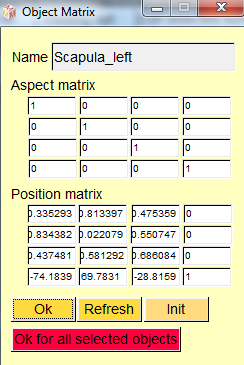
\includegraphics[scale=0.5]{images/File/Position2.png}
 \captionof{figure}{Object matrix window}
 \end{minipage} 
\noindent


\section{Rendering modification}
\section{Scalar arrays}
\section{RGB arrays}
\section{Tag arrays}



%\section{Delete small objects.}


